\documentclass{report}

\usepackage{graphicx}
\usepackage{hyperref}
\usepackage{tikz}
\usepackage{pgfplots}
\usepackage{multirow}
\usepackage{tabulary}


\author{Mihalache Radu-Stefan}
\date{}
\title{}


\begin{document}
\begin{center}
\Large
\textbf{Study of function minima using Hill Climbing, Simulated Annealing and Genetic algorithms}
        
\vspace{0.4cm}
\textbf{Mihalache Radu Stefan}
       
\vspace{1.2cm}
\textbf{Abstract}

\end{center}

\vspace{0.4cm}
In this paper I will approach the problem of solving the global minima with Hill Climbing,  Simulated Annealing and Genetic algorithms,
use my implementation to compare their performance and draw some conclusions regarding their efficacy.


\section*{Introduction}
\subsection*{Motivation}
The problem of exploring the values of functions and finding the global minimum of said function for a specified domain has useful applications, yet it is difficult to solve with a deterministic algorithm.
That is because some functions have a very small accumulation basin compared with the size of the domain for the global minimum.

\begin{figure}[!h]
  \centering
\begin{tikzpicture}
  \begin{axis}[
      xlabel=x,
      ylabel=$f(x)$
    ]
    \addplot [
      color=red,
      mark=x
    ]
    coordinates {
      (0, 5)
      (1, 5.1)
      (2, 5.2)
      (3, 5.3)
      (3.3, 0)
      (3.5, 5.4)
      (7, 5.5)
    };
  \end{axis}
\end{tikzpicture}
\end{figure}
\pagebreak

To solve this problem we will explore the following nondeterministic approaches:
\newline
\hspace*{10mm} - The Hill Climbing algorithm which is a greedy method
\newline
\hspace*{10mm} - The Simulated Annealing algorithm which is a meta-heuristic method that better explores the function's domain
\newline
\hspace*{10mm} - The Genetic algorithm which takes inspiration from nature and adapts its solution population to get closer to the global minimum
\newline
\newline
The motivation of this experiment is to determine which one of the approaches listed above gives 
the best results for a set of functions  in the shortest amount of time and examine why. 

\section*{Method}

The representation of the input variables will be a string of n bits such that they can adequately represent the function domain.

$$x = a + decimal_{represenation}(bit_{str}) \cdot (b - a)/(2^n - 1) ,  x \in \left[a, b \right]$$

Hill Climbing and Simulated annealing make use of this representation by generating a random input called the candidate solution, its vicinity can be explored by negating one bit, such that the hamming distance between the candidate solution and the vicinity is one.
\newline
\newline
\textbf{Hill Climbing}:
\newline
\newline
Selects a candidate solution for each iteration and try to improve it using either the first better vicinity (first improvement) or the best vicinity (best improvement). 
This algorithm finds the minimum by exploring the basin of the candidate solution.
\newline
\newline
\textbf{Simulated annealing}:
\newline
\newline
Selects a candidate solution at the start and explore its vicinity. This algorithm better explores the domain of the function by choosing worse vecinities based on the probability given by this expression:
\newline
$$random.uniform(0, 1) < math.exp(-abs((evaln - evalc) / temperature))$$
\newline
This algorithm makes use of the hot iron concept. At the beginning the temperature  is high and the chance to choose a worse solution is high, but it decreases over each iteration 
(which makes it more greedy)  based on this formula:
\newline
$$temperature = temperature \cdot 0.9$$

\pagebreak

\noindent
\textbf{Genetic}:
\newline
\newline
The genetic algorithm takes inspiration from nature, by holding a population of chromosomes, which are selected and evolve under the pressure a a fitness function.
A chromosome represents a potential solution and its chances to be selected for the next generation depend on the chromosome's evaluation by the fitness function.
As the solution is set of bits, a gene is an individual bit in the solution. The evolution process is accomplished by performing mutation and cross over on the chromosomes of the population.
\newline
\newline
Mutation is performed by flipping a random bit of a chromosome.
\newline
\newline
Crossover at one point between two chromosomes is performed by picking a random locus (position of a gene) and swapping the genes after the locus between the two. Example, locus = 4 :
$$10101010 \rightarrow 10101111 $$
$$11111111 \rightarrow 11111010 $$
\newline
The fitness function $fit(chromosome)$ that I have used in this experiment is inversely proportional with the result of the function $f(chromosome)$ for which we want to find the minima.
It uses $maximum = max(f(current_{population}))$ and $minimum = min(f(current_{population}))$ .
\newline
$$fit(chromosome) = (maximum - f(chromosome)) / (maximum- minimum)$$
\newline
The selection mechanism I have used in this experiment is Wheel of Fortune. It calculates the totalFitness
$$totalFitness = \sum(fit(chromosome))  , chromosome \in population$$
in order to compute the individual probability $p_{chromosome} = fit(chromosome) /  totalFitness$
and an array of cumulated probabilities $q_{i + 1} = q_{i} + p_{chromosome_i}$ that it uses to a chromosome at position $j$,  $population_{size}$ times such that:
$$r \in \left(0, 1 \right] \, , \, q_j < r < q_{j + 1}$$
\newline
An additional mechanism my genetic algorithm implementation make use of is Elitism. It makes sure that the best x solutions are always maintained in the population and mitigates the effects
of evolutions that do not result in better solutions.

\pagebreak

\section*{The analysed functions:}

\begin{figure}[!h]
  \centering
  $$ f(x) = \sum_{i=1}^n \left[ x_i^2 \right],
   x_i \in \left[ -5.12, 5.15 \right]$$
   $$min = 0$$

  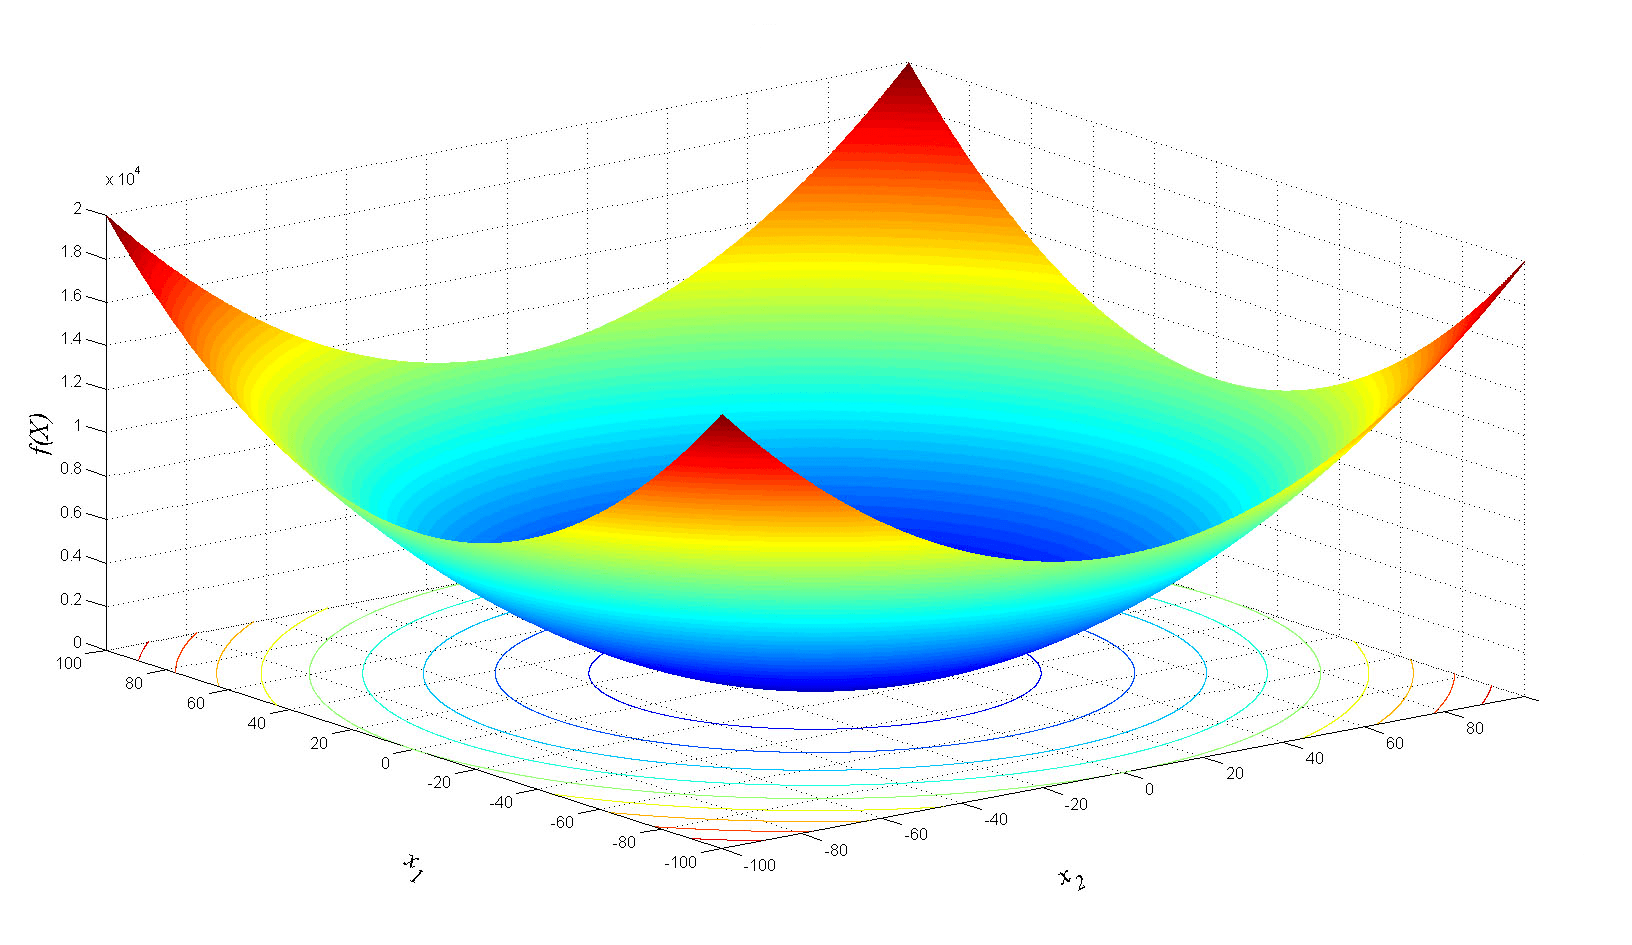
\includegraphics[width=100mm,scale=0.5]{De_Jong_function}
  \caption{Image De Jong's Function.\protect\footnotemark}
\end{figure}
\footnotetext{https://al-roomi.org/benchmarks/unconstrained/n-dimensions/}

\pagebreak

\begin{figure}[!h]
  \centering
  $$ f(x) = \sum_{i=1}^n \left[-x_i \cdot sin(sqrt(|x_i|)) \right],
   x_i \in \left[ -500, 500 \right]$$
   $$min = (-n) * 418.98$$

  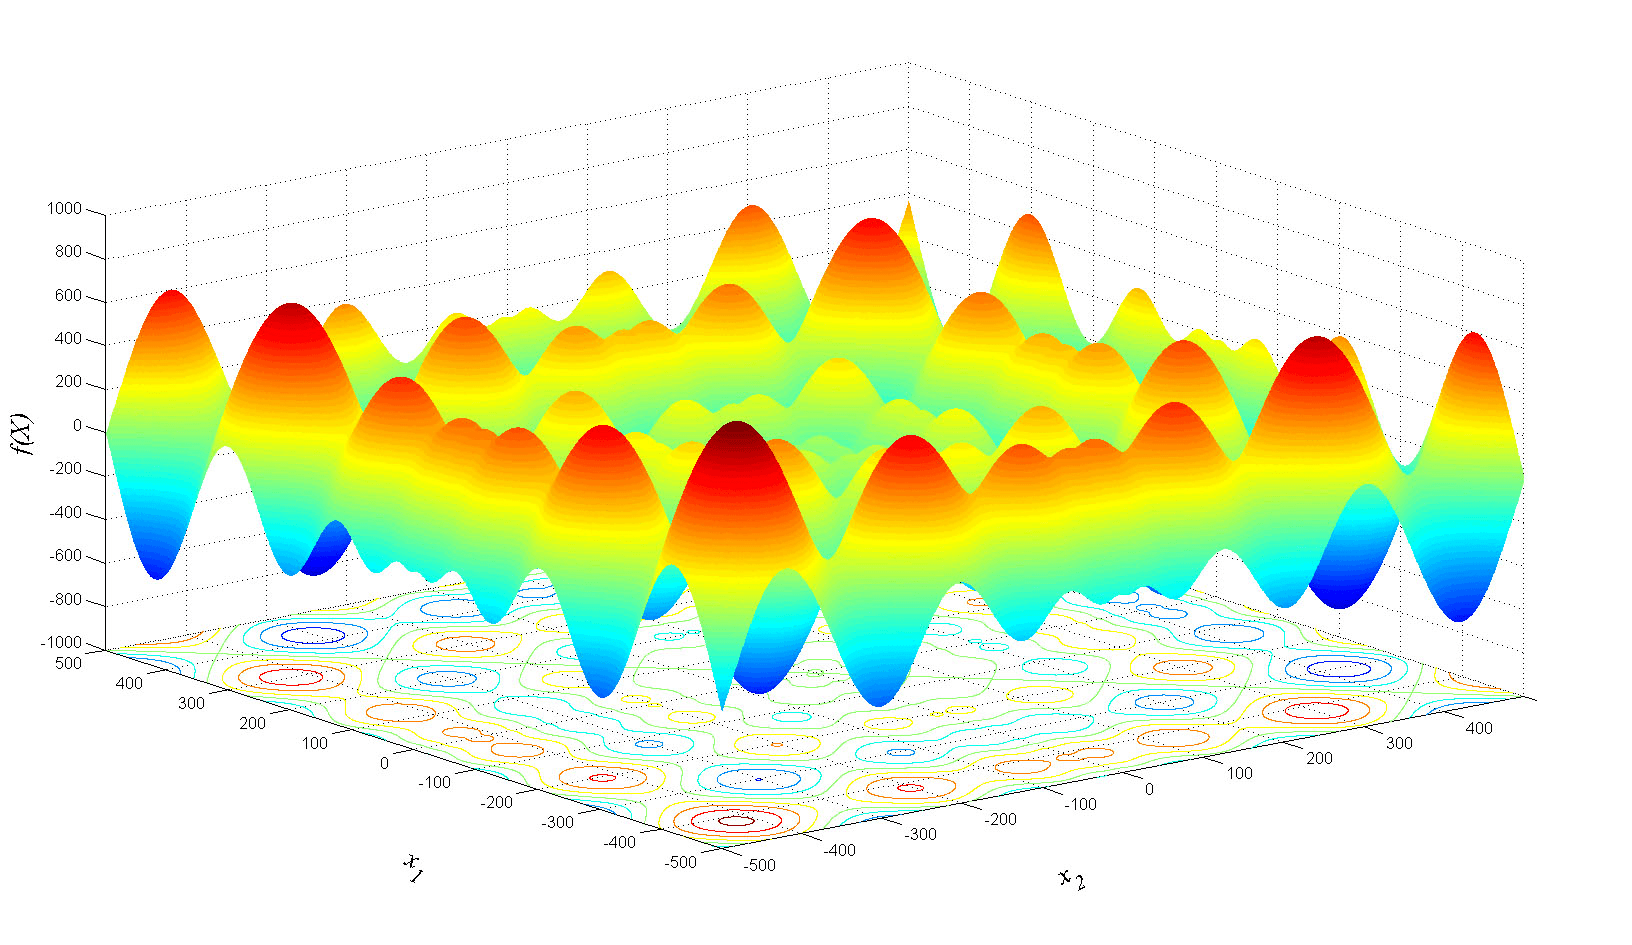
\includegraphics[width=100mm,scale=0.5]{Schwefel_fucntion}
  \caption{Image Schwefel's Function. \protect\footnotemark}
\end{figure}
\footnotetext{https://al-roomi.org/component/tags/tag/schwefel-function}

\begin{figure}[!h]
  \centering
  $$ f(x) = A \cdot n + \sum_{i=1}^n \left[ x_i^2 - A \cdot cos(2 \pi x_i) \right],
  A = 10, x_i \in \left[ -5.12, 5.15 \right]$$
   $$min = 0$$

  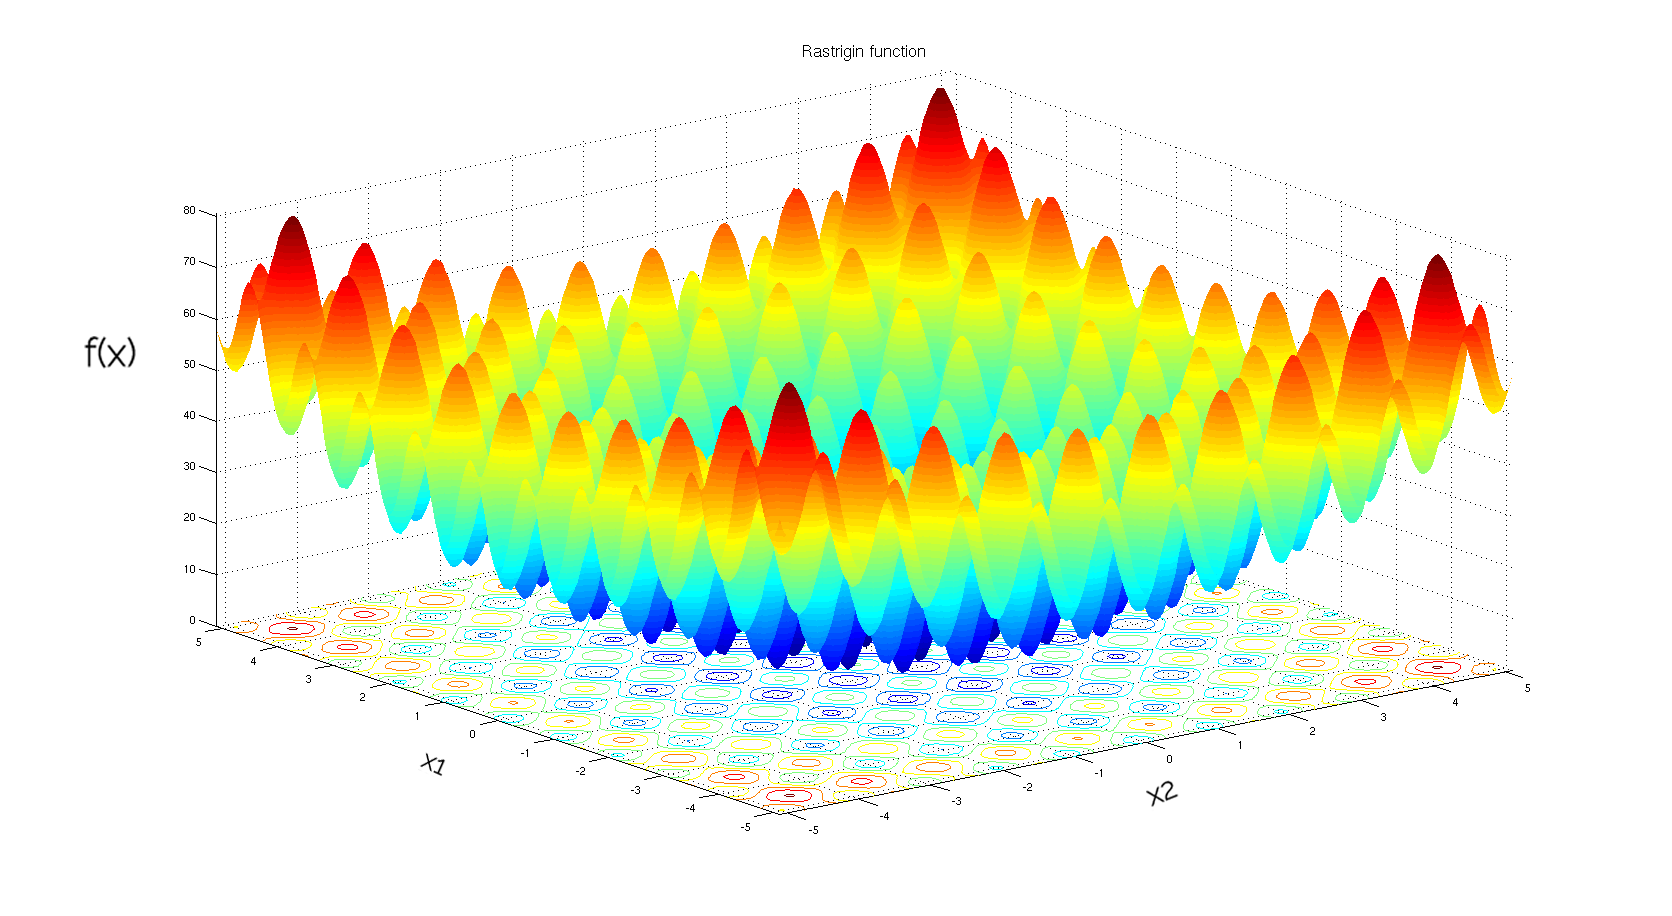
\includegraphics[width=100mm,scale=0.5]{Rastrigin_function}
  \caption{Image Rastrigin's Function. \protect\footnotemark}
\end{figure}
\footnotetext{https://commons.wikimedia.org/wiki/MainPage}

\pagebreak

\begin{figure}[!h]
  \centering
  $$ f(x) = -\sum_{i=1}^n \left[sin(x_i) \cdot \left( sin\left( \frac{i \cdot x_i^2}{\pi}  \right) \right)^{2 \cdot m} \right] ,
  x_i \in \left[ 0, \pi \right] ,  m = 10$$

   $$min = -4.68 \, , \, n = 5$$
   $$min = -9.66 \, , \, n = 10$$
   $$min < -27.5 \, , \, n = 30$$

  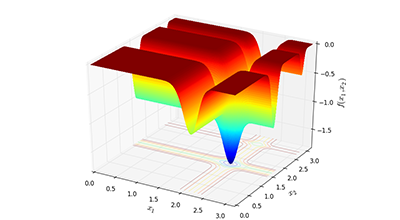
\includegraphics[width=100mm,scale=0.5]{Michalewicz_functions}
  \caption{Michalewicz's Function. \protect\footnotemark}
\end{figure}
\footnotetext{https://www.sfu.ca/~ssurjano/michal.html}

\pagebreak

\section*{Experiment}

The Hill Climbing and Simulate Anealing algorithms were implemented in python and analized the functions above with 100 iterations. The temperature for simulated aneealing is initially 2000.
\newline
The Genetic algorithm was implemented in C++ and analized the functions above with a population of 200, an elite population of 10 and 2000 iterations. The test was run on the compiled 64 bit program with -O2 compiler flag.
\newline
Each test has $10^{-5}$ precissionn is run 30 times to ensure consistency.

\section*{Results}

\begin{center}


$$DeJong \, 5D$$
\begin{tabulary}{1\textwidth}{|c|c|c|c|c|c|}
\hline
\multirow{2}{*}{Algorithms} & \multicolumn{4}{c|}{Solutions} & \multirow{2}{*}{Time Averege}
     \\
\cline{2-5}
 & Averege & Minimum &  Maximum &  S.D. &  \\
\hline
 H.C. First& 0 & 0 & 0 & 0 & 14 \\
\hline
 H.C. Best & 0 & 0 & 0 & 0 & 28  \\
\hline
 Simulated An. & 0 & 0 & 0 & 0 & 4  \\
\hline
 Genetic & 0 & 0 & 0 & 0 & 0.33 \\
\hline
\end{tabulary}


$$DeJong \, 10D$$
\begin{tabulary}{1\textwidth}{|c|c|c|c|c|c|}
\hline
\multirow{2}{*}{Algorithms} & \multicolumn{4}{c|}{Solutions} & \multirow{2}{*}{Time Averege}
     \\
\cline{2-5}
 & Averege & Minimum &  Maximum &  S.D. &  \\
\hline
 H.C. First& 0 & 0 & 0 & 0 & 112 \\
\hline
 H.C. Best & 0 & 0 & 0 & 0 & 216  \\
\hline
 Simulated An. & 0 & 0 & 0 & 0 & 8  \\
\hline
 Genetic & 0 & 0 & 0 & 0 & 0.49 \\
\hline
\end{tabulary}


$$DeJong \, 30D$$
\begin{tabulary}{1\textwidth}{|c|c|c|c|c|c|}
\hline
\multirow{2}{*}{Algorithms} & \multicolumn{4}{c|}{Solutions} & \multirow{2}{*}{Time Averege}
     \\
\cline{2-5}
 & Averege & Minimum &  Maximum &  S.D. &  \\
\hline
 H.C. First& 0 & 0 & 0 & 0 & 1946 \\
\hline
 H.C. Best & 0 & 0 & 0 & 0 & 2570  \\
\hline
 Simulated An. & 0 & 0 & 0 & 0 & 20  \\
\hline
 Genetic & 0 & 0 & 0 & 0 & 0.91 \\
\hline
\end{tabulary}

\pagebreak

$$Schwefel \, 5D$$
\begin{tabulary}{1\textwidth}{|c|c|c|c|c|c|}
\hline
\multirow{2}{*}{Algorithms} & \multicolumn{4}{c|}{Solutions} & \multirow{2}{*}{Time Averege}
     \\
\cline{2-5}
 & Averege & Minimum &  Maximum &  S.D. &  \\
\hline
 H.C. First& -1939 & -1992 & -1853 & 39.96799 & 22 \\
\hline
 H.C. Best & -1967 & -2094 & -1893 & 22.53137 & 20  \\
\hline
 Simulated An. & -1825 & -1963 & -1776  & 60.46418 & 6 \\
\hline
 Genetic & -2094.90312 & -2094.91443 & -2094.70647 & 0.04100 & 0.50 \\
\hline
\end{tabulary}


$$Schwefel \, 10D$$
\begin{tabulary}{1\textwidth}{|c|c|c|c|c|c|}
\hline
\multirow{2}{*}{Algorithms} & \multicolumn{4}{c|}{Solutions} & \multirow{2}{*}{Time Averege}
     \\
\cline{2-5}
 & Averege & Minimum &  Maximum &  S.D. &  \\
\hline
 H.C. First & -3652 & -3872 & -3492 & 75.35139 & 262 \\
\hline
 H.C. Best & -3623 & -3772 & -3506 & 64.45263 & 166  \\
\hline
 Simulated An. & 3642 & -3905 & -3246  & 235.82154 & 14  \\
\hline
 Genetic & -4189.45055 & -4189.82574  & -4189.20499 & 0.15884 & 0.69 \\
\hline
\end{tabulary}


$$Schwefel \, 30D$$
\begin{tabulary}{1\textwidth}{|c|c|c|c|c|c|}
\hline
\multirow{2}{*}{Algorithms} & \multicolumn{4}{c|}{Solutions} & \multirow{2}{*}{Time Averege}
     \\
\cline{2-5}
 & Averege & Minimum &  Maximum &  S.D. &  \\
\hline
 H.C. First & -9453 & -9923 & -9369 & 172.57403 & 3051 \\
\hline
 H.C. Best & -10153 & -10453 & -10063 & 149.3988 & 3022  \\
\hline
 Simulated An. & -9746  & -11279 & -9365  & 746.63063 & 40  \\
\hline
 Genetic & -12495.54426 & -12568.20105  & -12410.66695 & 49.48430 & 1.58773 \\
\hline
\end{tabulary}


$$Rastrigin \, 5D$$
\begin{tabulary}{1\textwidth}{|c|c|c|c|c|c|}
\hline
\multirow{2}{*}{Algorithms} & \multicolumn{4}{c|}{Solutions} & \multirow{2}{*}{Time Averege}
     \\
\cline{2-5}
 & Averege & Minimum &  Maximum &  S.D. &  \\
\hline
 H.C. First& 2.29497 & 1.58367 & 3.39702 & 0.64999 & 26 \\
\hline
 H.C. Best & 1.93592 & 1.279144 & 1.68702 & 0.2869 & 28  \\
\hline
 Simulated An. & 2.23086 & 1.71005 & 3.102193 & 1.20147 & 6  \\
\hline
 Genetic & 0 & 0 & 0 & 0 & 0.43 \\
\hline
\end{tabulary}


$$Rastrigin \, 10D$$
\begin{tabulary}{1\textwidth}{|c|c|c|c|c|c|}
\hline
\multirow{2}{*}{Algorithms} & \multicolumn{4}{c|}{Solutions} & \multirow{2}{*}{Time Averege}
     \\
\cline{2-5}
 & Averege & Minimum &  Maximum &  S.D. &  \\
\hline
 H.C. First& 7.18790 & 3.93217 & 15.19234 & 4.1881 & 322 \\
\hline
 H.C. Best & 8.18790 & 3.67834 & 14.0925 & 3.70173 & 242 \\
\hline
 Simulated An. & 9.18790 & 3.19593 & 15.2394 & 6.15804 & 14  \\
\hline
 Genetic & 0.23970 & 0 & 2.24758 & 0.56087 & 0.63 \\
\hline
\end{tabulary}

\pagebreak

$$Rastrigin \, 30D$$
\begin{tabulary}{1\textwidth}{|c|c|c|c|c|c|}
\hline
\multirow{2}{*}{Algorithms} & \multicolumn{4}{c|}{Solutions} & \multirow{2}{*}{Time Averege}
     \\
\cline{2-5}
 & Averege & Minimum &  Maximum &  S.D. &  \\
\hline
 H.C. First& 33.72184 & 27.12235 & 48.63187 & 7.93803 & 3234 \\
\hline
 H.C. Best & 32.43780 & 26.97201 & 47.29053 & 7.6298 & 2784  \\
\hline
 Simulated An. & 35.18790 & 27.67834 & 56.44140 & 10.8435 & 42  \\
\hline
 Genetic & 16.18794 & 6.32544 & 29.65766 & 5.57709 & 1.47341 \\
\hline
\end{tabulary}


$$Michalevicz \, 5D$$
\begin{tabulary}{1\textwidth}{|c|c|c|c|c|c|}
\hline
\multirow{2}{*}{Algorithms} & \multicolumn{4}{c|}{Solutions} & \multirow{2}{*}{Time Averege}
     \\
\cline{2-5}
 & Averege & Minimum &  Maximum &  S.D. &  \\
\hline
 H.C. First& -4.44109 & -4.62793 & -3.97123 & 0.24477 & 22 \\
\hline
 H.C. Best & -4.37306 &  -4.65685 & -4.02012 & 0.22591 & 20  \\
\hline
 Simulated An. & -4.28916 & -4.6328 & -3.26917 & 0.71647 & 4  \\
\hline
 Genetic & -4.69345 & -4.69346 & -4.69342 & 0.00013 & 0.68 \\
\hline
\end{tabulary}


$$Michalevicz \, 10D$$
\begin{tabulary}{1\textwidth}{|c|c|c|c|c|c|}
\hline
\multirow{2}{*}{Algorithms} & \multicolumn{4}{c|}{Solutions} & \multirow{2}{*}{Time Averege}
     \\
\cline{2-5}
 & Averege & Minimum &  Maximum &  S.D. &  \\
\hline
 H.C. First& -8.20880 & -9.01029 & -6.89132 & 0.76238 & 214 \\
\hline
 H.C. Best & -9.09037 &  -9.24031 & -8.25910 & 0.39391 & 158 \\
\hline
 Simulated An. & -8.70903 & -9.22690 &  -6.15737 & 1.51983 & 12 \\
\hline
 Genetic & -9.56998 & -9.66005 & -9.30496 & 0.09151 & 1.16 \\
\hline
\end{tabulary}


$$Michalevicz \, 30D$$
\begin{tabulary}{1\textwidth}{|c|c|c|c|c|c|}
\hline
\multirow{2}{*}{Algorithms} & \multicolumn{4}{c|}{Solutions} & \multirow{2}{*}{Time Averege}
     \\
\cline{2-5}
 & Averege & Minimum &  Maximum &  S.D. &  \\
\hline
 H.C. First& -20.79776 & -22.61219 & -17.31592 & 1.92739 & 1260 \\
\hline
 H.C. Best & -24.09166 & -25.14376 & -22.21472 & 1.05992 & 846  \\
\hline
 Simulated An. & -23.66259 & -24.29173 & -21.53991 & 3.8554 & 30 \\
\hline
 Genetic & -27.09429 & -28.04950 & -25.58877 & 0.59147 & 3.11664 \\
\hline
\end{tabulary}


\end{center}

\pagebreak

\section*{Analysing Results}
First of all, in regards to time this is not a fair comparison since the algorithms were implemented in different languages. 
\newline
\newline
In regards to the quality of the results given, the genetic algorithm scores better than all the other algorithms. This may be explained by the fact that it does 
not "blindly" search the domain on the function, like the others do in some manner, but always constructs the solutions based on what "already works" while still maintaining a great degree of freedom when exploring the function's domain.
\newline
\newline
Another aspect that can be observed is the fact that S.D. values for low number of axes is extremely low and it exponentially increases as the number of axes increases. While this is true for all algorithms, I have done some testing to see how the S.D. changes with more iterations
and found that it decreases significantly. 
\newline
\newline
I believe this signifies the fact that the genetic algorithm has somewhat steady progress towards an optimum solution and that with a certain number of iterations it will reach a good solution with a higher degree of probability than the other algorithms.

\section*{Conclusions}
First of all, the number of elite individuals assures that the best persist in the population, but also decreases the genetic diversity as the number of iterations increases. 
\newline
\newline
I tried to replicate this by lowering the number of cross-overs with the number of iterations, but the only function that was affected positively was the DeJong. From this, I can conclude that genetic diversity must be balanced with favoring better results.
\newline
\newline
In regards to the implementation details, increasing the efficiency of the algorithm greatly helped with testing and fine-tuning the algorithm.
In this sense I propose using std::bitset for representing the solutions and bitwise operations to evolve them and also do the operations with the chromosomes of the population on multiple threads.
\newline
\newline
\newline
\newline
\newline
\newline
\newline
\newline
\newline
I believe that, while the genetic algorithm scores the best in my implementation, it can benefit from some techniques used in the other algorithms, for example, after finding an elite member of the population it can be "enhanced" by applying one iteration of a Hill Climbing algorithm.
Also, to better emulate real conditions, a genetic algorithm may implement more than one population with different fitness functions with a chance for the populations to intersect at a certain number of iterations.

\begin{thebibliography}{9}

\bibitem{wikipedia}
  Wikipedia Commons \\ Rastrigin's Function rendered image.
  \url{https://commons.wikimedia.org/wiki/Main_Page}

\bibitem{Al-roomi}
  Al-roomi  \\ De Jong's Function rendered image.
  \url{https://al-roomi.org/benchmarks/unconstrained/n-dimensions/}
  Al-roomi  \\ Schwefel's Function rendered image.
  \url{https://al-roomi.org/component/tags/tag/schwefel-function}

\bibitem{Sfui}
   Sfu \\ Michalewicz's Function rendered image.  
\url{https://www.sfu.ca/~ssurjano/michal.html}


\bibitem{Geatbx}
  Geatbxi  \\ Function formulas.
  \url{http://www.geatbx.com/docu/fcnindex-01.html}

\bibitem{Course}
  Course Page.
  \url{https://profs.info.uaic.ro/~eugennc/teaching/ga/l}

\bibitem{Pycharm}
  Pycharm.
  \url{https://www.jetbrains.com/pycharm/}

\bibitem{Visual Studio}
  Visual Studio.
  \url{https://visualstudio.microsoft.com/}

\bibitem{Random function}
  Random function.
  \url{https://en.cppreference.com/w/cpp/numeric/random/uniform_int_distribution}

\end{thebibliography}  


\end{document}
